%%%%%%%%%%%%%%%%%%%%%%%%%%%%%%%%%%%%%%%%%
% Beamer Presentation
% LaTeX Template
% Version 1.0 (10/11/12)
%
% This template has been downloaded from:
% http://www.LaTeXTemplates.com
%
% License:
% CC BY-NC-SA 3.0 (http://creativecommons.org/licenses/by-nc-sa/3.0/)
%
%%%%%%%%%%%%%%%%%%%%%%%%%%%%%%%%%%%%%%%%%

%----------------------------------------------------------------------------------------
%	PACKAGES AND THEMES
%----------------------------------------------------------------------------------------

\documentclass{beamer}

\mode<presentation> {

% The Beamer class comes with a number of default slide themes
% which change the colors and layouts of slides. Below this is a list
% of all the themes, uncomment each in turn to see what they look like.

%\usetheme{default}
%\usetheme{AnnArbor}
%\usetheme{Antibes}
%\usetheme{Bergen}
%\usetheme{Berkeley}
%\usetheme{Berlin}
%\usetheme{Boadilla}
\usetheme{CambridgeUS}
%\usetheme{Copenhagen}
%\usetheme{Darmstadt}
%\usetheme{Dresden}
%\usetheme{Frankfurt}
%\usetheme{Goettingen}
%\usetheme{Hannover}
%\usetheme{Ilmenau}
%\usetheme{JuanLesPins}
%\usetheme{Luebeck}
%\usetheme{Madrid}
%\usetheme{Malmoe}
%\usetheme{Marburg}
%\usetheme{Montpellier}
%\usetheme{PaloAlto}
%\usetheme{Pittsburgh}
%\usetheme{Rochester}
%\usetheme{Singapore}
%\usetheme{Szeged}
%\usetheme{Warsaw}

% As well as themes, the Beamer class has a number of color themes
% for any slide theme. Uncomment each of these in turn to see how it
% changes the colors of your current slide theme.

%\usecolortheme{albatross}
%\usecolortheme{beaver}
%\usecolortheme{beetle}
%\usecolortheme{crane}
%\usecolortheme{dolphin}
%\usecolortheme{dove}
%\usecolortheme{fly}
%\usecolortheme{lily}
%\usecolortheme{orchid}
%\usecolortheme{rose}
%\usecolortheme{seagull}
%\usecolortheme{seahorse}
%\usecolortheme{whale}
%\usecolortheme{wolverine}

%\setbeamertemplate{footline} % To remove the footer line in all slides uncomment this line
%\setbeamertemplate{footline}[page number] % To replace the footer line in all slides with a simple slide count uncomment this line

%\setbeamertemplate{navigation symbols}{} % To remove the navigation symbols from the bottom of all slides uncomment this line
}

\usepackage{graphicx} % Allows including images
\usepackage{booktabs} % Allows the use of \toprule, \midrule and \bottomrule in tables

\usepackage[hangul]{kotex} % Korean support


\graphicspath{ {D:/_PlayGround/Github/2016_thesis/tex/images/} }









%----------------------------------------------------------------------------------------
%	TITLE PAGE
%----------------------------------------------------------------------------------------

\title[]{ADF 모의실험 및 비교} % The short title appears at the bottom of every slide, the full title is only on the title page

\author{김동완} % Your name
\institute[고려대학교 정책대학원] % Your institution as it will appear on the bottom of every slide, may be shorthand to save space
{
고려대학교 정책대학원\\ % Your institution for the title page
데이터 통계학과\\
\medskip
\textit{} % Your email address
}
\date{\today} % Date, can be changed to a custom date


\begin{document}

\begin{frame}
\titlepage % Print the title page as the first slide
\end{frame}

\begin{frame}
\frametitle{Overview} % Table of contents slide, comment this block out to remove it
\tableofcontents % Throughout your presentation, if you choose to use \section{} and \subsection{} commands, these will automatically be printed on this slide as an overview of your presentation
\end{frame}



%----------------------------------------------------------------------------------------
%	PRESENTATION SLIDES
%----------------------------------------------------------------------------------------

%------------------------------------------------
\section{개요} % Sections can be created in order to organize your presentation into discrete blocks, all sections and subsections are automatically printed in the table of contents as an overview of the talk
%------------------------------------------------

\subsection{문제점 분석} % A subsection can be created just before a set of slides with a common theme to further break down your presentation into chunks

\begin{frame}
\frametitle{문제점 분석}
\begin{itemize}

\item 지난달 구현에서의 문제점은 $\theta_{t}$ 의 예측분포를 update 해야하는데, $\theta_{t-1}$ 의 사후 분포를 update하여 생긴 문제로 보임. 이를 보완하기 위해 정규분포의 특성에 따라 $\sigma^2_{t,i}$를 update하는 단계에서 $\theta_{t}$의 분산을 더해줌. $\theta_{t}$의 분산 값으로는 iteration이 증가함에 따라 불확실성이 감소함을 반영하기 위해 $\theta_{t-1}$의 사후 평균의 절대값을 iteration 수로 나눈 값을 사용함.
\begin{eqnarray}
 \mu_{t,i} &=& \mu_{t|t-1,i} + a_i \delta_m
\\ \sigma^2_{t,i} &=& \sigma^2_{t-1,i} + a^2_i \delta_v + |\mu_{t,i}|/t
\\ a_i &\triangleq& \frac{x_{t,i}\sigma^2_{t|t-1,i}}{\sum_j x^2_{t,j}\sigma^2_{t|t-1,i}}
\end{eqnarray}

\end{itemize}
\end{frame}
%------------------------------------------------





%----------------------------------------------------------------------------------------
%	PRESENTATION SLIDES
%----------------------------------------------------------------------------------------

\subsection{실험 목적} % A subsection can be created just before a set of slides with a common theme to further break down your presentation into chunks

\begin{frame}
\frametitle{실험 목적}
\begin{itemize}
\item ADF(Assumed Density Filtering)를 GLM에 적용하는 것은 온라인 경사 하강법(Online Gradient Descent)과 많은 부분이 유사하며, 매 반복에서 선형식 $\eta$와 각 회귀 계수의 분포를 Step size에 반영하는 것이 차이점.
\item 모의 실험을 통해 로지스틱 회귀에 있어서 '온라인 경사 하강법'과 'ADF 방법'을 비교 하고자 함. 
\end{itemize}
\end{frame}

%------------------------------------------------





%----------------------------------------------------------------------------------------
%	PRESENTATION SLIDES
%----------------------------------------------------------------------------------------

\subsection{비교 대상 방법론} % A subsection can be created just before a set of slides with a common theme to further break down your presentation into chunks

\begin{frame}
\frametitle{비교 대상 방법론}
\begin{itemize}
\item 경사 하강법(Gradient Descent): 1차 최적화 알고리즘 중 하나로 함수의 극솟값(local minimum) 및 값수값이 극솟값을 갖게 하는 모수를 점진적으로 찾는 방법
\item 배치 경사 하강법(Batch Gradient Descent): 매 반복(iteration)마다 전체 데이터를 사용하여 극솟값을 찾는 방법
\item 온라인 경사 하강법(Online Gradient Descent): 매 반복에서 하나의 셈플을 사용하여 극솟값을 찾는 방법
\end{itemize}
\end{frame}

%------------------------------------------------






%----------------------------------------------------------------------------------------
%	PRESENTATION SLIDES
%----------------------------------------------------------------------------------------

%------------------------------------------------
\section{모의 실험} % Sections can be created in order to organize your presentation into discrete blocks, all sections and subsections are automatically printed in the table of contents as an overview of the talk
%------------------------------------------------

\subsection{모의 데이터} % A subsection can be created just before a set of slides with a common theme to further break down your presentation into chunks


\begin{frame}
\frametitle{모의 데이터}
\begin{itemize}
\item 아래 조건으로 단순 로지스틱 회귀모형을 위한 데이터를 3000건 생성.\\
$\qquad logit(E[Y_i]) = w_{0i} + w_{1i} x_{1i}, \quad i=1, ..., n$  \\
$\qquad w_{0i} \overset{i.i.d}{\sim} N(3,1), \quad i=1, ..., n$ \\
$\qquad w_{1i} \overset{i.i.d}{\sim} N(10,1), \quad i=1, ..., n$ \\
$\qquad y_i \sim Bern(p_i =logit^{-1}(w_{0i} + w_{1i} x_{1i})), \quad i=1, ..., n$

\item 경사하강법(GD)에서 사용할 step size $\alpha$값은 $w_0$에는 0.08, $w_1$에는 1.1을 사용.

\end{itemize}
\end{frame}
%------------------------------------------------






%----------------------------------------------------------------------------------------
%	PRESENTATION SLIDES
%----------------------------------------------------------------------------------------

\subsection{회귀 계수 추정: 최대 우도} % A subsection can be created just before a set of slides with a common theme to further break down your presentation into chunks


\begin{frame}
\frametitle{회귀 계수 추정: 최대 우도}
\begin{itemize}
\item 전체 데이터를 이용하여 회귀 계수($w_{0i}, w_{1i}$)에 대한 최대 우도 추정치를 구하면 아래와 같다.\\

%\begin{center}
%\includegraphics[scale=0.7]{mle001.eps}
%\end{center}

\begin{center}
\begin{tabular}{l l l}
\toprule
\textbf{회귀 계수} & \textbf{추정치} & \textbf{P-value}\\
\midrule
$w_0(intercept)$ 	& 2.6620 & $<$2e-16 \\
$w_1$ 						& 8.6870 & $<$2e-16 \\
\bottomrule
\end{tabular}
\end{center}

\end{itemize}
\end{frame}
%------------------------------------------------





%----------------------------------------------------------------------------------------
%	PRESENTATION SLIDES
%----------------------------------------------------------------------------------------

\subsection{모의 실험 결과: $w_0$} % A subsection can be created just before a set of slides with a common theme to further break down your presentation into chunks


\begin{frame}
\frametitle{모의 실험 결과: $w_0$}

\begin{itemize}
\item iteration이 증가함에 따른 $w_0$(intercept) 값의 변화 비교 \\
(온라인 경사하강법(GD) vs ADF)
\begin{center}
\includegraphics[scale=0.55]{sim_w0_v001.eps} %730 * 430
\end{center}

\end{itemize}
\end{frame}
%------------------------------------------------






%----------------------------------------------------------------------------------------
%	PRESENTATION SLIDES
%----------------------------------------------------------------------------------------

\subsection{모의 실험 결과: $w_1$} % A subsection can be created just before a set of slides with a common theme to further break down your presentation into chunks


\begin{frame}
\frametitle{모의 실험 결과: $w_1$}

\begin{itemize}
\item iteration이 증가함에 따른 $w_1$(intercept) 값의 변화 비교 \\
(온라인 경사하강법(GD) vs ADF)
\begin{center}
\includegraphics[scale=0.55]{sim_w1_v001.eps} %730 * 430
\end{center}

\end{itemize}
\end{frame}
%------------------------------------------------




%----------------------------------------------------------------------------------------
%	PRESENTATION SLIDES
%----------------------------------------------------------------------------------------

\subsection{모의 실험 결과: 비교} % A subsection can be created just before a set of slides with a common theme to further break down your presentation into chunks


\begin{frame}
\frametitle{모의 실험 결과: 비교(1)}

\begin{itemize}
\item 두 방법 모두 iteration이 증가함에 따라 MLE 추정치로 근사함을 알 수 있고, ADF의 경우 초기 각 계수의 큰 분산의 영향으로 그 변위 폭이 GD에 비해 큼을 알 수 있다.
\begin{table}
\begin{tabular}{l l l}
\toprule
\textbf{Iteration} & \textbf{GD} & \textbf{ADF} \\
\midrule
 200 & 0.2071293 & 0.1498564 \\
 500 & 0.1632435 & 0.1278876 \\
1500 & 0.1493539 & 0.1335120 \\
3000 & 0.1441112 & 0.1352678 \\
\bottomrule
\end{tabular}
\caption{$\frac{Log loss}{iteration}$}
\end{table}


\end{itemize}
\end{frame}
%------------------------------------------------




%----------------------------------------------------------------------------------------
%	PRESENTATION SLIDES
%----------------------------------------------------------------------------------------

\begin{frame}
\frametitle{모의 실험 결과: 비교(2)}

\begin{itemize}
\item 두가지 방법론에서 iteration 당 log-loss를 비교해 보면 아래와 같고, ADF가 약간 더 좋은 결과를 보임을 알 수 있다. 그러나 iteration이 많아 지면 그 차이가 점차 줄어들게 된다.

\begin{center}
\includegraphics[scale=0.55]{sim_loss_v001.eps} %730 * 430
\end{center}


\end{itemize}
\end{frame}
%------------------------------------------------





%------------------------------------------------

\begin{frame}
\frametitle{References}

\footnotesize{
\begin{thebibliography}{99} % Beamer does not support BibTeX so references must be inserted manually as below

\bibitem[오만숙., 2012]{p1} 오만숙, (2012)
\newblock R몬테칼로와 함께하는 베이지안 통계추론
\newblock \emph{자유아카데미} Ch17, p115 - 116.

\bibitem[Murphy, K.P., 2012]{p1} Murphy, K.P.(2012)
\newblock Machine learning
\newblock \emph{The MIT Press} Ch18.5.3, p652 - 655.

\bibitem[Zoeter, O., 2007]{p1} Zoeter, O. (2007)
\newblock Bayesian Generalized Linear Models in a Terabyte World.
%\newblock \emph{The MIT Press} Ch18.5.3, p652 - 655.


\end{thebibliography}
}

\end{frame}

%------------------------------------------------

\begin{frame}
\Huge{\centerline{The End}}
\end{frame}

%----------------------------------------------------------------------------------------

%
% Reference
%


\end{document} 